\centering
\resizebox{\linewidth}{!}{
\begin{tikzpicture}

\node (sample) at (-6,0) {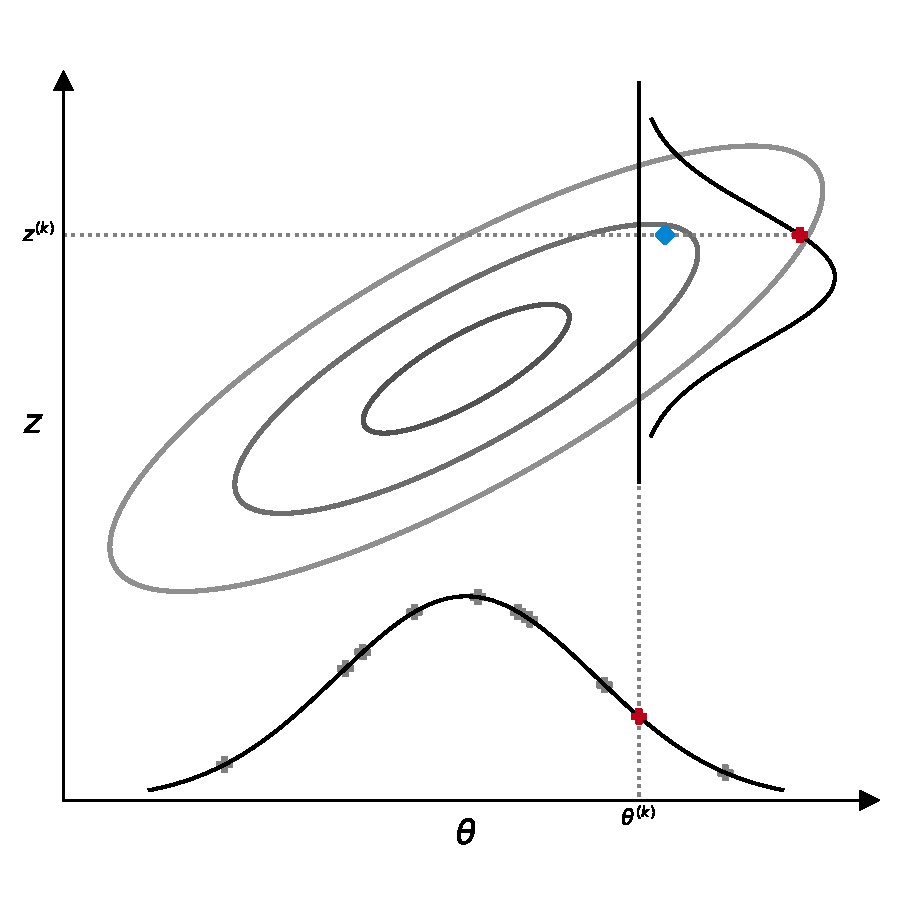
\includegraphics[width=3.25cm]{joint_dist_sampling.pdf}};

\node at (-3,-0.75) {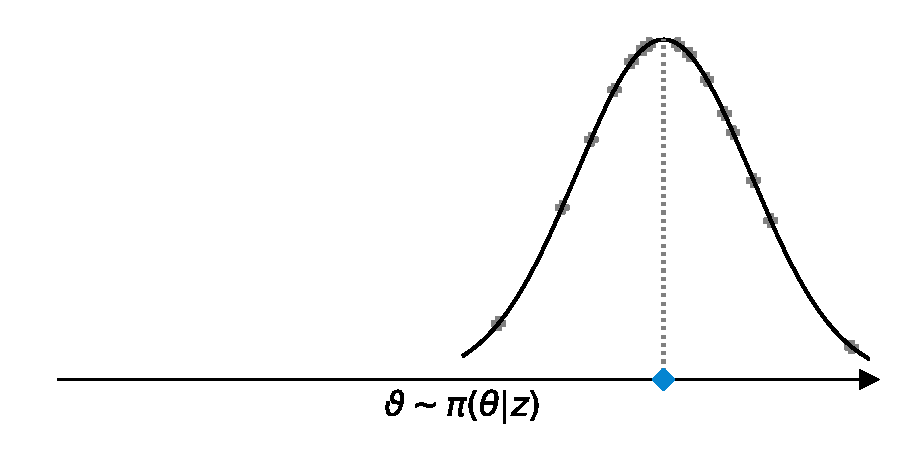
\includegraphics[width=2cm]{posterior_dist_sampling.pdf}};
\node at (-3,0.5) {\large Guess};

\begin{scope}
\clip (0,0) circle (1.25cm);
\node[circle, fill=white, minimum width=2.5cm] at (0,0) {};
\node (lp) at (0,0) {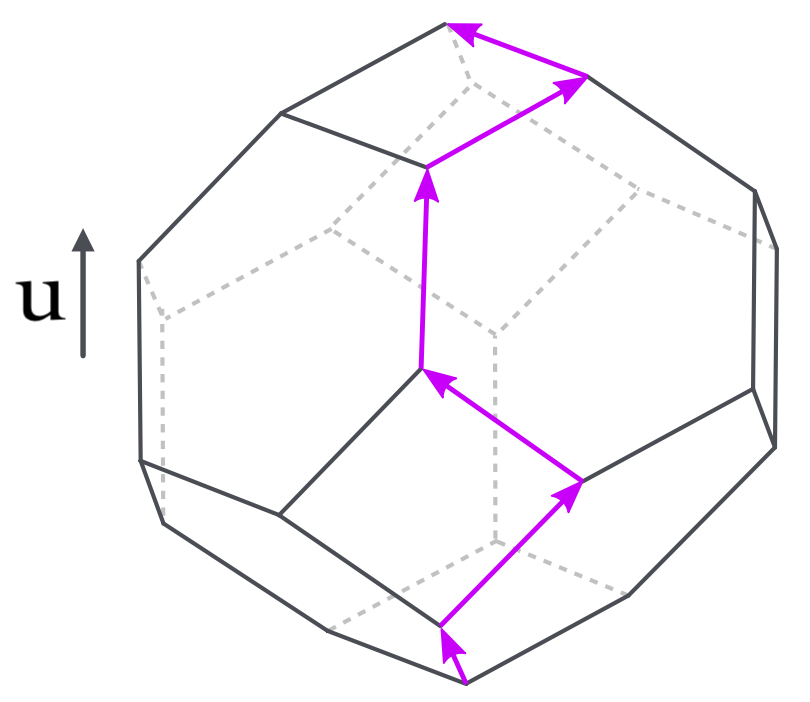
\includegraphics[width=2.3cm]{lp.png}};
\end{scope}

\node at (0, -1.65) {\large Decide};

\node at (2.6,0.5) {\large Imagine};

\node[rectangle, fill=white, minimum width=3.7cm, minimum height=1.9cm, rounded corners=7.5pt] (eval_bg) at (6,0) {};
\node (eval) at (6,0) {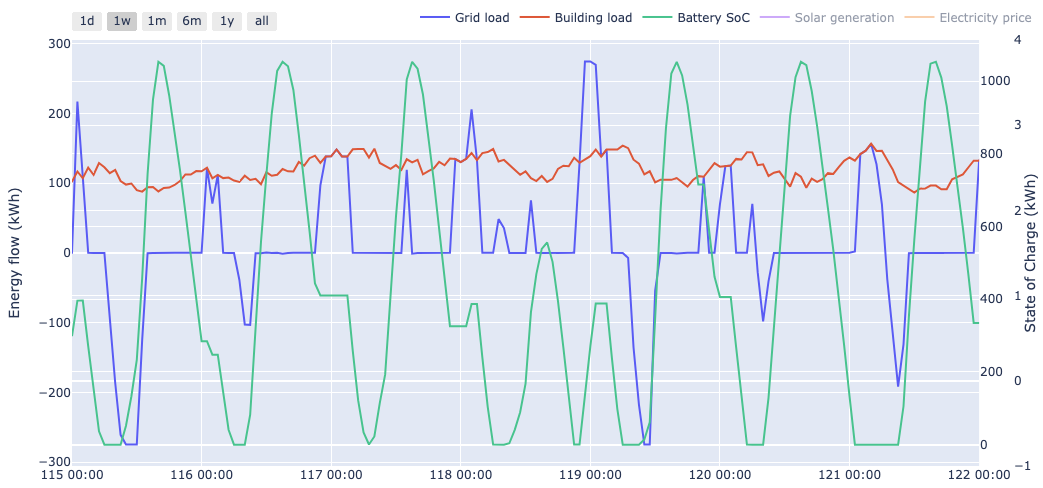
\includegraphics[width=3.5cm]{sim.png}};
\node[xshift=0.4cm, yshift=-0.45cm] (kpi) at (eval_bg.north west) {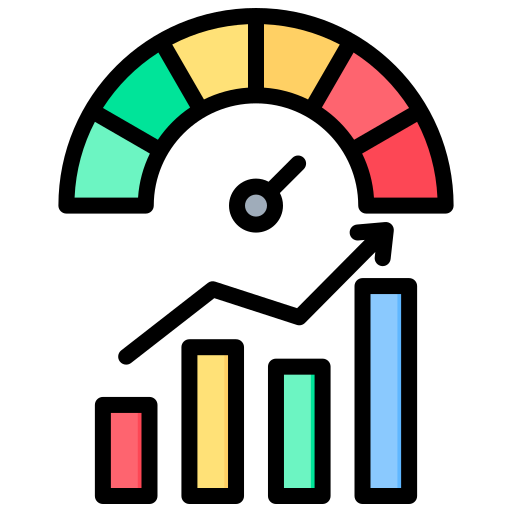
\includegraphics[width=0.65cm]{kpi.png}};

\node[align=right] at (4.8, -2.75) {\large Repeat};

\node[circle, fill=white, minimum width=1.25cm] (sigma) at (0,-3.25) {\HUGE $\mathlarger{\Sigma}$};

\begin{scope}[line width=.8mm, color=gray!75!black, arrows={-Stealth[inset=0pt, angle=60:10pt]}]
    \draw[shorten <= -2mm, shorten >= 1mm] (sample) -- (lp);
    \draw[shorten <= 1mm, shorten >= 1mm] (lp) -- (eval);
    \draw[shorten <= 1.5mm, shorten >= 1mm] (eval) |- (sigma);
    \draw[dashed, shorten <= 1mm, shorten >= -1.5mm] (sigma) -| (sample);
\end{scope}

\end{tikzpicture}
}